\documentclass{beamer}
 
\usepackage[utf8]{inputenc}
 
 
%Information to be included in the title page:
\title{Hacking Medical Devices for Fun and Insulin: Breaking the Human 
SCADA System}
\subtitle{Analisi delle vulnerabilità negli Infusori}
\author{Francesco Montelli}
\institute{CeSeNa}
\date{2017}
 
 
 
\begin{document}
 
\frame{\titlepage}

\begin{frame}
\frametitle{Considerazioni iniziali}
	\begin{itemize}
		\item Deve funzionare 24/7
		\item E' in grado di ricevere le misurazioni del CGM
		\item Disponibile un controllo remoto per somministrare insulina
		\item Porta USB per programmare l'infusore e scaricare dati
		\item Pensato per durare nel tempo, aggiornamenti quasi totalmente assenti
	\end{itemize}
\end{frame}

\begin{frame}
\frametitle{Analisi}
	\begin{itemize}
		\item Comunicazini più complesse
		\item Programmi di configurazioni antiquati, basati su XP
		\item Nel programma di configurazione è possibile impostare la quantità dele informazioni di log su HIGH
	\end{itemize}
\end{frame}

\begin{frame}
\frametitle{Analisi dei log}
	\begin{figure}
		\centerline{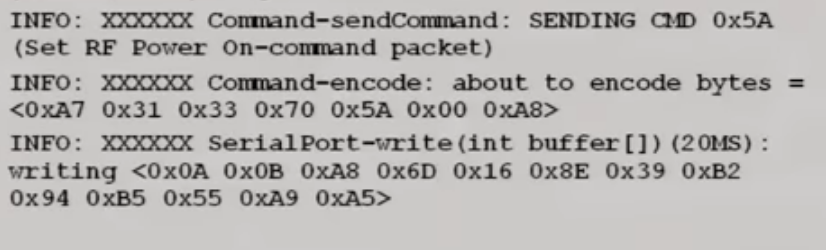
\includegraphics[scale=0.4]{log}}
		\caption{esempio di cattura di un pacchetto}
	\end{figure}
\end{frame}

\begin{frame}
\frametitle{Analisi del file Jar}
	\begin{itemize}
		\item Comunica direttamente sulla posta seriale
		\item Non offuscato
		\item Mostra in chiaro l'implementazione di *ogni* comando
		\item Mostra la struttura di ogni pacchetto
	\end{itemize}
\end{frame}

\begin{frame}
\frametitle{Analisi dell'infusore}
	\begin{itemize}
		\item{Impossibilità di disattivare il controllo remoto}
		\item{Nessuna convalida dei comandi ricevuti}
		\item{Deve essere configurate per consentire al dispositivo di contrllo di inviare comandi}
	\end{itemize}
\end{frame}

\begin{itemize}
\frametitle{HW necessario}
	\begin{itemize}
		\item Trasmettitore radio USB
		\item Comando remoto per infusore (acquistabile senza prescrizione medica)
	\end{itemize}
\end{itemize}



\end{document}